\documentclass{article}

%% preamble
\usepackage{hyperref}
\usepackage{verbatim}
\usepackage{color}
\usepackage{graphicx}
\usepackage{amsmath}
\usepackage{amsfonts}
\usepackage{cancel}

\topmargin 0pt
\advance \topmargin by -\headheight
\advance \topmargin by -\headsep
\textheight 9.in
\oddsidemargin 0pt
\evensidemargin \oddsidemargin
\marginparwidth 0.5in
\textwidth 6.5in
\newcommand{\myhrule}{ \begin{center}\rule{.9\linewidth}{.25mm}\end{center} }
\definecolor{darkgray}{rgb}{0.95,0.95,0.95}
\definecolor{heavygray}{rgb}{0.05,0.05,0.05}
\definecolor{foo}{rgb}{.8,0,.8}
\newcommand{\pad}{\vspace{8pt}\noindent}
\newcommand{\red}[1]{{\color{red}#1\color{black}}}
\newcommand{\myhref}[2]{\href{#1}{\color{foo}\underline{#2}\color{black}}}

\newcommand{\Mod}[1]{\ \mathrm{mod}\ #1}


\begin{document}

\title{CMDA 3634 Spring 2018 Homework 05}

%% change this to your name
\author{Pim Silpacharn}
\vspace{-64pt}\maketitle
\begin{center}\underline{You must complete the following task by 5pm on Tuesday 04/24/18.}\end{center}
Your write up for this homework should be presented in a {\LaTeX} formatted PDF document. You may copy the \LaTeX{} used to prepare this report as follows

\begin{enumerate}
\item Click on this  \myhref{https://www.sharelatex.com/read/cyvqcnwmfnsc}{link} 
\item Click on Menu/Copy Project.
\item Modify the HW05.tex document to respond to the following questions. 
\item Remember: click the Recompile button to rebuild the document when you have made edits.
\item Remember: Change the author. 

\end{enumerate}

\pad \emph{Each student} must individually upload the following files to the CMDA 3634 Canvas page at \myhref{https://canvas.vt.edu}{https://canvas.vt.edu}

\begin{enumerate}
\item \verb|firstnameLastnameHW05.tex| {\LaTeX} file.
\item Any figure files to be included by \verb|firstnameLastnameHW05.tex| file.
\item \verb|firstnameLastnameHW05.pdf| PDF file.
\end{enumerate}

\noindent In addition, all source code must be submitted to an online git repository as follows:
\begin{enumerate}
    \item While on the webpage for your git repository, go to Settings $\rightarrow$ Collaborators.
    \item Add nchalmer@vt.edu and zjiaqi@vt.edu as collaborators. 
    \item Make a folder named HW05 in you repository and store all relevant source files to this assignment in this folder. Ensure your assignment files compile with {\verb make }.
\end{enumerate}

\pad You must complete this assignment on your own.

\vspace{16pt}
\begin{center}
\underline{\bf 100 points will be awarded for a successful completion.}
\vspace{8pt}\underline{\bf Extra credit will be awarded as appropriate.}
\end{center}

\newpage


\section*{ElGamal Public-key Cyptography}

Through the previous assignments, we've manged to develop a functional program which performs encryption and decryption of string messages using an $n$ bit ElGamal cryptographic system. We can set up the cryptographic system by finding the values of the public key $(p,g,h)$. We can cast characters in strings into elements of $\mathbb{Z}_p$ and encrypt them. Finally, we can decrypt elements of $\mathbb{Z}_p$ and cast them back to characters if we know the secret key $x$. 

In the case where we imagined that we do not have access to the secret key $x$, we have used MPI and OpenMP to crack our ElGamal encryption in parallel using many CPU cores. Even with that level of parallelism, it is easy to see that our program can use $n$ bit encryption where $n$ is large enough that we still cannot find the secret key in a practical amount of time. 

In this final assignment, let's turn our previous monolithic programs into something a bit more useful by separating the basic operations into their own programs which run and save their results in files. Once we've accomplished that, let's tackle our final hurdle and use GPU acceleration to enable us to break even the strongest encryption our program can produce, namely $n=31$ bit cryptographic systems.


\pad {\bf Part 1: Setup, Encrypt, and Decrypt}

In the HW05 folder of the instructor's github the {\verb makefile } has been altered so that four separate programs will be compiled when you type {\verb make } or {\verb make } {\verb all }. The names of the programs are {\verb setup }, {\verb encrypt }, {\verb decrypt }, and {\verb cudaDecrypt }. They can be compiled separately by typing {\verb make } {\verb setup }, {\verb make } {\verb encrypt }, etc. Note that the function {\verb cudaDecrypt } requires CUDA's {\verb nvcc } compiler, and therefore the New River cluster, to compile. 

\vspace*{1em}
\noindent{\bf Q1}(10 points) The program in {\verb setup.c } is meant to perform the ElGamal cryptosystem setup routines and write the public key information to a file named {\verb public_key.txt }. Complete the program so that, after querying the user for a bit length $n$, it write the bit length $n$, prime $p$, generator $g$, and number $h$, to a file named {\verb public_key.txt }. For example, after running {\verb setup }, the file {\verb public_key.txt } could look something like,
\begin{verbatim}
    25
    30080879
    28192225
    28973487
\end{verbatim}
Which means $n=25$, $p=30080879$, $g=28192225$, and $h=28973487$.

\vspace*{1em}
\noindent{\bf Q2}(20 points) The program in {\verb encrypt.c } is meant to input a message string from the user and use the public key information in the file {\verb public_key.txt } to encrypt the message. Edit the program so that it after reading the message as a string from the user the program reads the public key information from {\verb public_key.txt } and encrypts the message. Afterwards, write the the number of cyphertext pairs, and each cyphertext pair $(\hat{m},a)$, into a file called {\verb message.txt }. The contents of {\verb message.txt } should look something like,
\begin{verbatim}
    14
    28395666 9350445
    3562739 5794092
    10156865 16818778
    2858293 6363325
    29107964 21484289
    3274137 24856781
    19487449 15592980
    18341691 30012651
    15930624 18293246
    11025926 2833780
    3862999 23130298
    16935347 23161724
    21230787 9009798
    25866655 2102881
\end{verbatim}
which indicates that there are 14 cyphertext entries, $(\hat{m},a)_1 = (28395666,9350445)$, $(\hat{m},a)_2 = (3562739,$ $5794092)$, etc. 

\vspace*{1em}
\noindent{\bf Q3.1}(20 points) The program in {\verb decrypt.c } is meant to read the contents of {\verb public_key.txt } and {\verb message.txt } and decrypt the message. After reading the files, the program will ask the user for the secret key. Complete the program so that if the user inputs $x=0$ or an incorrect secret key, the program will attempt to break the encryption by searching for the correct secret key $x$. Once the correct secret key is found, decrypt the contents of {\verb message.txt } and print the message to the terminal. 

\noindent{\bf Q3.2}(5 points) Using the {\verb decrypt } function or one of your programs from previous assignments, give a rough estimate of how long you would expect a serial code to break an $n=31$ bit encryption. Be sure to explain how you arrived at your estimate. 


\pad {\bf Part 2: GPU Accelerated Decryption}
In this part, we will use Nvidia's CUDA programming language to add GPU acceleration to the {\verb decrypt } function. In the HW05 folder is the CUDA file {\verb cudaDecrypt.cu }. Begin this section by copying the contents of the {\verb main } function in your complete {\verb decrypt.c } file to to {\verb cudaDecrypt.cu }


\vspace*{1em}
\noindent{\bf Q4.1}(10 points) Examine the loop where we search for the secret key. Describe in words how/why we could perform this section of the program in a GPU kernel. What would the kernel require as input? How much output will the kernel produce, and how do we access it on the host? How much memory must we allocate on the device? How many threads per block would be reasonable? Why?

\vspace*{1em}
\noindent{\bf Q4.2}(35 points) Edit the {\verb cudaDecrypt.cu } file to implement the kernel you described in Q4.1, i.e. add a GPU kernel function which can find the secret key $x$. If any {\verb __device__ } functions are required add them to {\verb cudaDecrypt.cu } as well (you may need to rename them to not conflict with functions in {\verb functions.c }). Be sure to {\verb cudaMalloc } any arrays the kernel will need, and use {\verb cudaMemcpy } to transfer memory between host and device.

\vspace*{1em}
\noindent{\bf Q4.3}(5 points) Experiment with decrypting several different $n$-bit encryptions. In general, how much faster (in time and throughput) is the GPU accelerated version of your decryption program? Assuming you could scale perfectly in parallel with MPI or OpenMP, how many CPU cores would you need in order to achieve the same performance as one of the P100 GPUs on the New River cluster?

\vspace{5mm}
Answer: The GPU accelerated version of the decryption program is significantly faster. You would need a lot of cores in order to match the P100 GPU's performance. 

\vspace{5mm}
\noindent{\bf Bonus:}(20 points) In the HW05 folder of the instructor's github there is a file named {\verb bonus_public_key.txt } and {\verb bonus_message.txt }. Decrypt the message and include a screenshot of the output here. 


\begin{figure}[h] 
    \centering
    \caption{Bonus Output}
    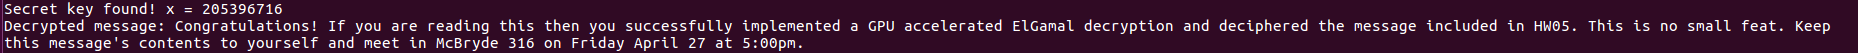
\includegraphics[scale = 0.75]{bonus.PNG}
\end{figure}
%\myhrule

%\begin{thebibliography}{9}
%\bibitem{gol} Wikipedia -- description of the Game of Life
%\url{https://en.wikipedia.org/wiki/Conway's_Game_of_Life}
 
%\end{thebibliography}


\end{document}